The following section provides details in the construction of the model for predicting stock prices, as well as a breakdown of the data used in the training of the network.

\section{Time-Series Forecasting}
Financial data are discrete in time and as such can be modelled as time-series with calculated means and standard deviations.

* time series analysis\\
* exploratory analysis
\section{Autoregressive Models}

\section{Model Description}
The network is a relatively simple network by most accounts, comprised of a single hidden layer. The simplicity of the model only goes to show the power of neural networks in fitting and forecasting time-series. The model consists of three layers, an input layer, a Long Short-Term Memory (LSTM) layer and the output layer, as shown in \ref{tab:model_arch}.

\begin{figure}[h]
    \centering
    \begin{neuralnetwork}[height=4]
        \newcommand{\x}[2]{$x_#2$}
        \newcommand{\y}[2]{$\hat{y}_#2$}
        \newcommand{\h}[2]{$h_#2$}
        \newcommand{\hlast}[2]{\ifnum4=#2 \vdots \else \ifnum5=#2 $h_{100}$ \else $h_#2$ \fi \fi}
        \inputlayer[count=4, bias=false, title=Input, text=\x]
        \hiddenlayer[count=5, bias=false, title=LSTM, text=\hlast] \linklayers
        \outputlayer[count=4, title=Output, text=\y] 
        \linklayers
    \end{neuralnetwork}
    \caption{Model Architecture}
    \label{tab:model_arch}
\end{figure}

The input layer receives a 2-dimensional array of historical stock values, including the previous day's opening, highest, lowest and closing stock prices. The network then allows the neurons to compete amongst each other and determing an appropriate output. Output is in the shape of a 1-dimensional array containing four values, the future day's predicted stock values for open, high, low and close. The LSTM layer contains 100 nodes and is trained for 100 epochs. The Rectifier Linear Unit was used as its activation function and the Mean Absolute Error was used as its loss function.

\begin{table}[h]
    \centering
    \begin{tabular}{|l|l|l|l|l|l|}
        \hline
        \textbf{Nodes} & \textbf{Epochs} & \textbf{Optimizer} & \textbf{Learning Rate} & \textbf{Activation} & \textbf{Loss} \\ \hline
        100            & 100             & Adam               & 0.001                  & ReLU                & MAE           \\ \hline
        \end{tabular}
    \caption{Description of the hidden LSTM layer}
    \label{tab:lstm_layer}
\end{table}

In this project we made use of the Keras API to implement the network. Keras is written in Python and operates ontop of TensorFlow, which is an extremely popular and widely used Deep Learning library. A simple sequential model using LSTM cells built using Keras would look like this:

\begin{minted}[mathescape, linenos, numbersep=5pt, gobble=2, frame=lines, framesep=2mm]{python}
    model = Sequential()
    model.add(LSTM(100, activation="relu", input_shape=(n_steps, n_features)))
    model.add(Dense(n_features))
    opt = Adam(learning_rate=0.001)
    model.compile(optimizer=opt, loss="mae", metrics=["mse"])
\end{minted}

With as little as 5 lines of code, we have a working Long Short-Term Memory model ready for training. The LSTM cell easily remembers the long term dependencies in the data and outputs a 1-dimensional array containing future values.


Here is a sentence, and you can see a nice picture in Figure \ref{fig:brayford}.

\begin{figure}[ht]
    \centering
    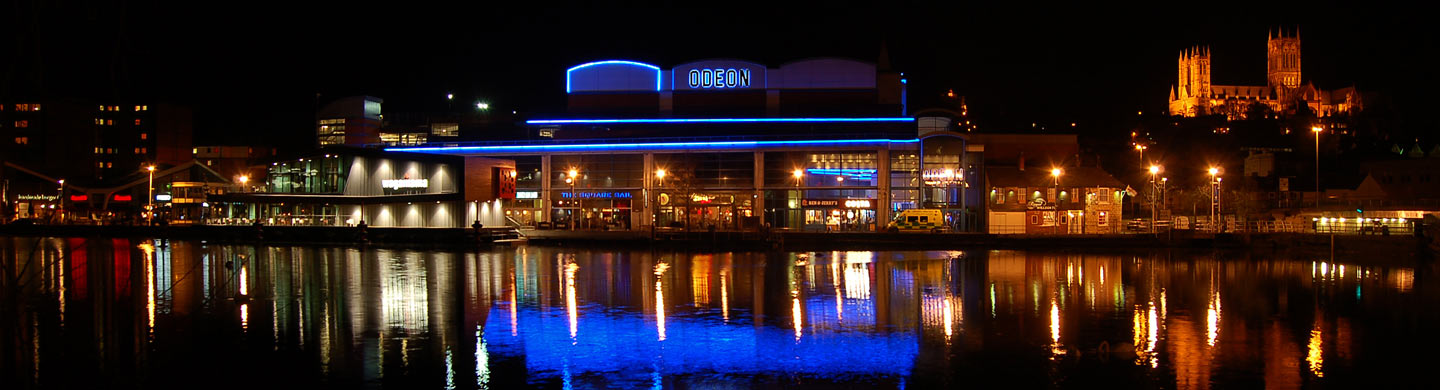
\includegraphics[width=\textwidth]{figures/brayford.jpg}
    \caption{A picture of the Brayford from Google Images.}
    \label{fig:brayford}
\end{figure}

Also, a table can be found in Table \ref{tbl:example-table}. You should use a \LaTeX~table generator like \url{https://www.tablesgenerator.com/} if you want to make your life easier.

\begin{table}[ht]
    \caption{Here is a table. The caption goes above like this.}
    \centering
    \begin{tabular}{l|l|c}
        First name & Last name & Age \\
        \hline\hline
        Bob & Bobbington & 24 \\
        Joe & Bloggs & 37 \\
        Billy & Bob & 10 \\

    \end{tabular}
    \label{tbl:example-table}
\end{table}